\documentclass[main.tex]{subfiles}
\begin{document}
\section{Fourier变换的引入}
对于周期为$2L$的周期函数,或定义在$\left[-L,L\right]$上的函数$f\left(x\right)$,其\emph{Fourier级数(Fourier series)}展开\cite[\S 11.5, \S 11.6]{华工高数2009下}形如
\begin{align}\label{eq:fourier_series_1}
    f\left(x\right)=\frac{1}{2}a_0+\sum_{n=1}^\infty a_n\cos\left(\frac{n\pi x}{L}\right)+b_n\sin\left(\frac{n\pi x}{L}\right)
\end{align}
其中
\begin{align*}
    a_n & =\frac{1}{L}\int_{-L}^L f\left(x\right)\cos\left(\frac{n\pi x}{L}\right)dx,                   \\
    b_n & =\frac{1}{L}\int_{-L}^L f\left(x\right)\sin\left(\frac{n\pi x}{L}\right)dx,\quad n=1,2,\cdots
\end{align*}
利用欧拉公式\footnote{正体小写字母$\I$专门用于表示虚数$\I\equiv\sqrt{-1}$。}
\begin{align*}
    \cos\left(x\right) & =\frac{1}{2}\left(e^{\I x}+e^{-\I x}\right)   \\
    \sin\left(x\right) & =\frac{1}{2\I}\left(e^{\I x}-e^{-\I x}\right)
\end{align*}
式\eqref{eq:fourier_series_1}可表示为
\begin{align}\label{eq:fourier_series_2}
    f\left(x\right) & =\sum_{n=-\infty}^{\infty}c_ne^{\I n\pi x/L},\quad c_n=\frac{1}{2L}\int_{-L}^Lf\left(x\right)e^{-\I n\pi x/L}dx
\end{align}
其中$c_0=\frac{1}{2}a_0,c_n=\left(a_n-\I b_n\right)/2,c_{-n}=\left(a_n+\I b_n\right)/2=\overline{c_n}$。

函数可作Fourier展开(或说式\eqref{eq:fourier_series_1}或式\eqref{eq:fourier_series_2}等号右边的Fourier级数收敛)的条件——\emph{狄利克雷条件(Dirichlet conditions)},请自行回顾\cite[定理11.6.1,p.301]{华工高数2009下}。

若$f\left(x\right)$定义在$\mathbb{R}$上,则至少可考虑$f$限制在在区间$\left(-L,L\right)$上的函数$f_L:\left(-L,L\right)\rightarrow\mathbb{R},f_L\left(x\right)=f\left(x\right)$的Fourier级数,它将形如式\eqref{eq:fourier_series_2}。我们进一步进行如下处理:
\begin{align*}
    f_L\left(x\right)         & =\sum_{n=-\infty}^\infty c_ne^{-\I n\pi x/L}                                                                                         \\
                              & =\sum_{n=-\infty}^\infty\left(\frac{1}{2L}\int_{-L}^L f_L\left(x^\prime\right)e^{-\I n\pi x^\prime/L}dx^\prime\right)e^{\I n\pi x/L} \\
    \left(\frac{n}{2L}\right. & \equiv \left.y_n,\Delta y=y_{n+1}-y_n=\frac{1}{2L}\right)                                                                            \\
                              & =\sum_{n=-\infty}^\infty\left[\int_{-L}^Lf_L\left(x^\prime\right)e^{-\I 2\pi y_nx^\prime}dx^\prime\right]e^{\I 2\pi xy_n\Delta y}
\end{align*}
让$L\rightarrow\infty$,与此同时$\Delta y\rightarrow 0$,在黎曼积分可积条件下,上式可记作以下积分
\begin{align}\label{eq:fourier_transform_1}
    f\left(x\right) & =\int_{-\infty}{\infty}dy\left[\int_{-\infty}^\infty dxf\left(x\right)e^{-\I 2\pi yx}\right]e^{\I 2\pi xy}dy \\
                    & =\int_{-\infty}^\infty dy\tilde{f}\left(y\right)e^{\I 2\pi xy}
\end{align}
其中
\[\tilde{f}\left(y\right)=\int_{-\infty}^\infty dxf\left(x\right)e^{-\I 2\pi yx}\]
称$f\left(x\right)$的\emph{Fourier变换(Fourier transform)},$f\left(x\right)$称$\tilde{f}\left(y\right)$的\emph{反Fourier变换(inverse Fourier transform)},记为
\[\tilde{f}\left(y\right)=\mathcal{F}\left\{f\left(x\right)\right\},\quad f\left(x\right)=\mathcal{F}^{-1}\left\{\tilde{f}\left(y\right)\right\}\]

函数$f\left(x\right)$存在Fourier变换的充份条件(需同时满足):
\begin{enumerate}
    \item $f\left(x\right)$绝对可积,即$\int_{-\infty}^{\infty}\left|f\left(x\right)\right|dx<\infty$
    \item $f\left(x\right)$在$\mathbb{R}$的任一有限区间上具有有限个极值
    \item $f\left(X\right)$在$\mathbb{R}$的任一有限区间上具有有限个不连续点,且在这些点上$f\left(x\right)$取有限函数值。
\end{enumerate}
等价地,可以说连续函数或具有有限个不连续点的有界函数存在Fourier变换。

定义在$\mathbb{R}^n$上的函数$f:\mathbb{R}^n\rightarrow\mathbb{R}$的Fourier变换形如:
\begin{equation}\label{eq:fourier_transform_2}
    f\left(\mathbf{x}\right)=\frac{1}{\left(2\pi\right)^n}\int_{\mathbb{R}^n}d\mathbf{k}\tilde{f}\left(\mathbf{k}\right)\exp\left(\I \mathbf{k}\cdot\mathbf{x}\right)
\end{equation}
其中
\[\tilde{f}\left(\mathbf{k}\right)=\int_{\mathbb{R}^n}d\mathbf{x}f\left(\mathbf{x}\right)\exp\left(-\I\mathbf{k}\cdot\mathbf{x}\right)\]
$f$的Fourier变换存在的条件与上述$n=1$的条件相似。

以下是一些常用的Fourier变换性质:
\begin{enumerate}
    \item 线性。若$h\left(x\right)=\alpha f\left(x\right)+g\left(x\right)$则$\tilde{h}\left(k\right)=\alpha\tilde{f}\left(k\right)+\tilde{g}\left(k\right),\forall \alpha\in\mathbb{R}$
    \item 时移。若$h\left(x\right)=f\left(x-x_0\right)$,则$\tilde{h}\left(k\right)=e^{-\mathrm{i}kx_0}\tilde{f}\left(k\right),\forall x_0\in\mathbb{R}$。
    \item 频移(调制)。若$h\left(x\right)=e^{-\mathrm{i}k_0x}f\left(x\right)$,则$\tilde{h}\left(k\right)=\tilde{f}\left(k-k_0\right),\forall k_0\in\mathbb{R}$。
    \item 时域标度。若$h\left(x\right)=f\left(\alpha x\right)$,则$\tilde{h}\left(k\right)=\left|\alpha\right|^{-1}\tilde{f}\left(k\right),\forall \alpha\neq 0$。
    \item 微分。$\mathcal{F}\left\{\frac{d}{dx}f\left(x\right)\right\}=\mathrm{i}k\mathcal{F}\left\{f\left(x\right)\right\},\quad\mathcal{F}\left\{\frac{d^n}{dx^n}f\left(x\right)\right\}=\left(\mathrm{i}k\right)^n\mathcal{f}\left\{f\left(x\right)\right\}$
    \item 卷积。若$h\left(x\right)=\int_{-infty}^\infty\overline{f\left(x^\prime\right)}g\left(x+x^\prime\right)dx^\prime$称为$f\left(x\right)$与$g\left(x\right)$的\emph{卷积(convolution)},则$\tilde{h}\left(k\right)=\tilde{f}\left(k\right)\tilde{g}\left(k\right)$。
\end{enumerate}

常见函数的Fourier变换对,可查Fourier变换表。

% =================================================
\section{狄拉克$\delta$函数}
\emph{狄拉克$\delta$函数(Dirac's $\delta$-function)}$\delta\left(x\right)$(简称$\delta$函数)是一个\emph{广义函数(generalized function)}\footnote{本讲义不对广义函数进行正式的定义。读者只需要了解$\delta$函数的基本性质就可以了。广义函数在数学上又称作\emph{分布(distributions)},可参考\cite{Richards1990}。}。设定义在$\mathbb{R}$上的任一实值函数$f\left(x\right)$任意整数阶可微,且在$\mathbb{R}$的某一有界闭集外处处为零,则$\delta\left(x\right)$必须满足性质
\begin{equation}\label{eq:dirac_delta_1}
    \int_{-\infty}^{\infty}\delta\left(x\right)f\left(x\right)dx=f\left(0\right)
\end{equation}
特别地,若取$f\left(x\right)=1$,则有
\begin{equation}\label{eq:dirac_delta_2}
    \int_{-\infty}^\infty\delta\left(x\right)dx=1
\end{equation}

在狭义定义下的函数当中,是不存在满足上述性质的函数的。但$\delta\left(x\right)$可通过常规函数序列引入。考虑以下函数序列(图\ref{fig:delta_series})
\[f_n\left(x\right)=\left(\frac{n}{\pi}\right)^{1/2}e^{-nx^2},\quad n\in\mathbb{N}\]
则
\begin{equation}\label{eq:dirac_series_conv}
    \delta\left(x\right)=\lim_{n\to\infty}f_n\left(x\right)
\end{equation}
确实,
\[\int_{-\infty}^{\infty}dxf_n\left(x\right)=1,\quad\forall n\in\mathbb{N}\]
故由式\eqref{eq:dirac_series_conv}和极限与积分的相关性质有
\[\int_{-\infty}^\infty\delta\left(x\right)dx=1\]
满足\eqref{eq:dirac_delta_2}。

\begin{figure}[ht]
    \centering
    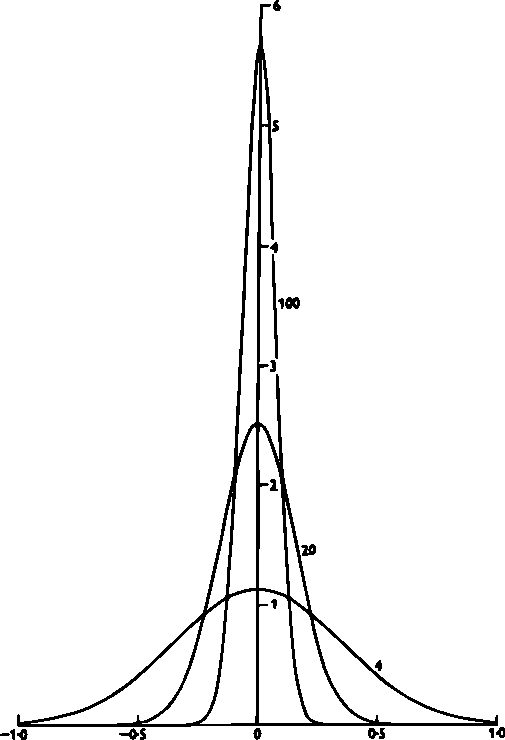
\includegraphics{../images/delta_series.pdf}
    \caption{函数序列$f_n\left(x\right)=e^{-nx^2}\left(\frac{n}{\pi}\right)^{1/2}$在$n=4,20,100$时的图像\cite{lighthill_1958}。}
    \label{fig:delta_series}
\end{figure}

要验证式\eqref{eq:dirac_series_conv}还一般地满足\eqref{eq:dirac_delta_1},我们需要证明
\[\lim_{n\to\infty}\int_{-\infty}^\infty dxf_n\left(x\right)f\left(x\right)=f\left(0\right)\]
对$f\left(x\right)$关于$x=0$进行泰勒展开\footnote{函数$f$满足的性须使其必可进行泰勒展开。}:
\[f\left(x\right)=\sum_{m=0}^\infty\frac{f^{\left(m\right)}\left(0\right)}{m!}x^m\]
故
\begin{align*}
    \lim_{n\to\infty}\int_{-\infty}^\infty dxf_n\left(x\right)f\left(x\right) & =\sum_{m=0}^\infty\frac{f^{\left(m\right)}\left(0\right)}{m!}\lim_{n\to\infty}\int_{-\infty}^\infty dxf_n\left(x\right)x^m                                                 \\
                                                                              & =\sum_{m=0}^\infty\frac{f^{\left(m\right)}\left(0\right)}{m!}\left[1+\left(-1\right)^m\right]\frac{\Gamma\left(\frac{m+1}{2}\right)}{2\sqrt{\pi}}\lim_{n\to\infty}n^{-m/2} \\
                                                                              & =f\left(0\right)
\end{align*}
上式只有$m=0$项不为零,故\eqref{eq:dirac_delta_1}得验。

利用式\eqref{eq:dirac_delta_1}和式\eqref{eq:dirac_delta_2},还可得到$\delta$函数的以下基本性质:
\begin{equation}\label{eq:delta_offset}
    \int_{-\infty}^\infty f\left(x\right)\delta\left(x-a\right)=\int_{-\infty}^\infty f\left(u+a\right)\delta\left(u\right)du=f\left(a\right)
\end{equation}
以及$\delta$函数的导数的性质(分部积分):
\begin{align}\label{eq:delta_derivative}
    \int_{-\infty}^\infty\frac{d}{dx}\delta\left(x\right)f\left(x\right)dx & =\left.f\left(x\right)\delta\left(x\right)\right|_{-\infty}^\infty-\int_{-\infty}^\infty f^\prime\left(x\right)\delta\left(x\right)dx\nonumber \\
                                                                           & =-f^\prime\left(0\right)
\end{align}
其中由于前面提到$f\left(x\right)$在$\mathbb{R}$的某一有界闭集外处处为零故$\lim_{x\to\pm\infty}f\left(x\right)=0$,上式的第一个等号右边的第一项为零(利用$\delta$函数与$f_n$的关系可验)。

以上仅以某一个函数序列在$n\rightarrow\infty$的极限规定了$\delta$函数,使得我们能够推导很多$\delta$函数的性质,但具有同样性质(式\eqref{eq:dirac_delta_1}和\eqref{eq:dirac_delta_2})的$\delta$函数可由不止一组函数序列来得到,这些函数序列在得出同一个$\delta$函数这件事上是等价的。只要一个函数序列$f_n\left(x\right)$对每一$n\in\mathbb{N}$满足:
\begin{enumerate}
    \item 关于$x=0$对称;
    \item 在$n\rightarrow\infty$时变得“无限高”和“无限窄”;
    \item 在$n\rightarrow\infty$时积分面积恒为1,
\end{enumerate}
则$\delta\left(x\right)=\lim_{n\to\infty}f_n\left(x\right)$就是狄拉克$\delta$函数。例如,另一个可得到$\delta$函数的等价函数序列是
\[
    g_n\left(x\right)=\left\{\begin{array}{ll}
        n, & -\frac{1}{2n}\leq x\leq\frac{1}{2n} \\
        0, & \text{otherwise}\end{array}\right.
\]

在$\mathbb{R}^n$上,可定义$n$维$\delta$函数$\delta\left(\mathbf{x}\right)=\prod_{i=1}^n\delta\left(x_i\right),\quad \mathbf{x}=\left(x_1,\cdots,x_n\right)$。此时,对任一定义在$\mathbb{R}^n$上的无穷阶可微且在$\mathbb{R}^n$的某有界闭集外处处为零的函数$f\left(\mathbf{x}\right)$有
\begin{equation}\label{eq:dirac_delta_3}
    \int_{\mathbb{R}^n}d\mathbf{x}\delta\left(\mathbf{x}-\mathbf{a}\right)f\left(\mathbf{x}\right)=f\left(\mathbf{a}\right)
\end{equation}

% =================================



\end{document}
